\documentclass[UTF8]{ctexart}
\usepackage{geometry}
\usepackage{indentfirst}
\usepackage{hyperref}
\usepackage{harpoon}
\usepackage{amsmath}
\usepackage{graphicx}
\usepackage{float}
\usepackage{subfigure}
\usepackage{multirow}
\usepackage{array}
\usepackage{tikz}
\usetikzlibrary{arrows, shapes, positioning, calc}
\geometry{a4paper, left=1cm, right=1cm, top=2cm, bottom=2cm}
\setlength{\parindent}{1cm}
\renewcommand\contentsname{Content}
\title{伊辛模型}
\author{段元兴}
\date{\today}
\begin{document}
\maketitle
\thispagestyle{empty}
\setcounter{page}{1}
\newpage
\tableofcontents
\newpage
    \section{提醒}
        \indent 这个大作业是由我之前的一次计算模拟改编而成的, 所以计算的内容不尽相同, 请见谅, 但是计算和优化的核心思想是掌握了的, 即蒙特卡洛-梅特波利斯方法和
        提高并行计算效率的方法.
    \section{计算方法}
        \indent 由于CPU计算的过于缓慢, 所以采用了GPU的CUDA来加速计算. 而这个问题对于使用double随机数的要求不高, 所以使用float随机数没有很大的影响.\\
        \indent 整体采用了并行计算模型, 其方式为: 将自旋格点取为unsigned long long数据的一位, 利用多个线程对互不相邻的格点进行操作, 这样理论上2次运算就能
        将整个网格都操作一遍, 极大的提高了效率. 将这样的2次运算作为一次迭代, 而一般迭代1000000次就能保证收敛.
    \section{计算结果}
        \indent 这里将对不同尺寸 (边长$2^k$, $k=7,8,9,10$) 的周期边界正方形网格进行计算, 统计出各个物理量随着温度$T$, 磁场强度$H$的变化情况 (为了避免网格大小造成的绝对值变化,
        以下的各个物理量都已经除以了格点数量), 观察其热容, 磁化率和熵, 以及网格尺寸, 温度和平均时间对于零外场临界相变磁畴凝聚的影响和模拟磁滞曲线.
        \subsection{磁矩和能量}
            \subsubsection{磁矩$M$}
                \indent 这是边长256网格的$M(H,T)$图像:
                \begin{center}
                    \includegraphics[width=17cm]{M-HT256.pdf}
                \end{center}
                可以在温度低于临界温度$T_c=2.268K$时发现明显的$M$不连续现象, 即意味着降温系统发生相变时磁矩的最终朝向是取决于外场方向的.\\
                \indent 而为了研究无外场下$T_c$附近磁矩与温度的关系, 经过提高分辨率和更多系统的平均, 并使用多次计算结果的平均, 得到以下结果:
                \begin{center}
                    \includegraphics[width=10cm]{PhaseTransition.pdf}
                \end{center}
                \newpage
            \subsubsection{能量$E$}
                \indent 这是边长256网格的$E(H,T)$图像:
                \begin{center}
                    \includegraphics[width=17cm]{E-HT256.pdf}
                \end{center}
                这里发现系统能量随着温度的增加, 在$T_c$以下系统能量基本不变, 而在$T>T_c$时整个系统的能量开始迅速增加, 且这个增加的速率会随着磁场的增强减小, 物理上理解就是
                外场强行把整个系统的磁矩作用成与磁场同向的, 系统处于低能态, 所以需要更高的温度以增大磁矩翻转的概率, 使系统的能量增加. 从等能曲线上也能看出, 相同的能量下,
                磁场强度越强, 温度越高, 而且一系列等能曲线中间出现了一个分叉点, 那个点的温度就是$T_c$, 物理含义: 从该点开始系统能量若要继续降低, 则磁场 (即系统磁矩) 的方向必须是
                一个确定的方向, 即发生了相变.
                \newpage
            \subsubsection{网格尺寸的影响}
                \indent 为了观察尺寸对于模拟的影响, 这里作出相对于边长128网格各个尺寸网格的$M, E$绝对差值:
                \begin{figure}[H]
                    \centering
                    \subfigure{\includegraphics[width=5.5cm]{DeltaM-HT256.pdf}}\quad
                    \subfigure{\includegraphics[width=5.5cm]{DeltaM-HT512.pdf}}\quad
                    \subfigure{\includegraphics[width=5.5cm]{DeltaM-HT1024.pdf}}\quad
                    \subfigure{\includegraphics[width=5.5cm]{DeltaE-HT256.pdf}}\quad
                    \subfigure{\includegraphics[width=5.5cm]{DeltaE-HT512.pdf}}\quad
                    \subfigure{\includegraphics[width=5.5cm]{DeltaE-HT1024.pdf}}\quad
                \end{figure}
                可以看出误差基本上是在$10^{-3}$级, 而且这个误差还会随着系综平均的数量的增加而减小, 所以可以认为这几个尺寸网格计算得到的$M, E$是基本一致的. 这种性质要归功于
                周期性, 即使网格不够大也能被其周期性弥补而不至于受到边界条件的过大影响.
                \newpage
        \subsection{热容, 磁化率和熵}
            \subsubsection{热容}
                \indent $H=0.1$T的热容计算结果如下:
                \begin{center}
                    \includegraphics[width=13cm]{Cv-T.pdf}
                \end{center}
                可以看出在$T_c$附近有热容的极值.
            \subsubsection{磁化率}
                \indent $H=0.1$T得磁化率计算结果如下:
                \begin{center}
                    \includegraphics[width=13cm]{Chi-T.pdf}
                \end{center}
            \subsubsection{熵}
                \indent $H=0.1$T的熵计算结果如下:   
                \begin{center}
                    \includegraphics[width=13cm]{S-T.pdf}
                \end{center}
                这与系综理论得到的无穷温度下的熵为$Nk\ln 2$吻合得非常好.
                \newpage
        \subsection{零外场磁畴凝聚}
            \indent 在临界相变的温度下, 系统会出现类似小磁畴的现象, 即一团相邻的格点磁矩方向相同. 这种现象的出现与磁矩相互作用的局域性有关, 即近邻的磁矩 (铁磁性) 在低温时会趋向于
            同向而使能量最低, 但是这种凝聚会被高温激发翻转磁矩破坏.
            \subsubsection{网格尺寸对零外场磁畴凝聚的影响}
                \indent 猜想这种凝聚现象与网格尺寸有关. 为模拟一定时间下的平均, 这里取了10个紧邻系统 (通过连续翻转自旋得到) 的平均. 以下是4个尺寸下在温度为2.3K的凝聚现象:
                \begin{center}
                    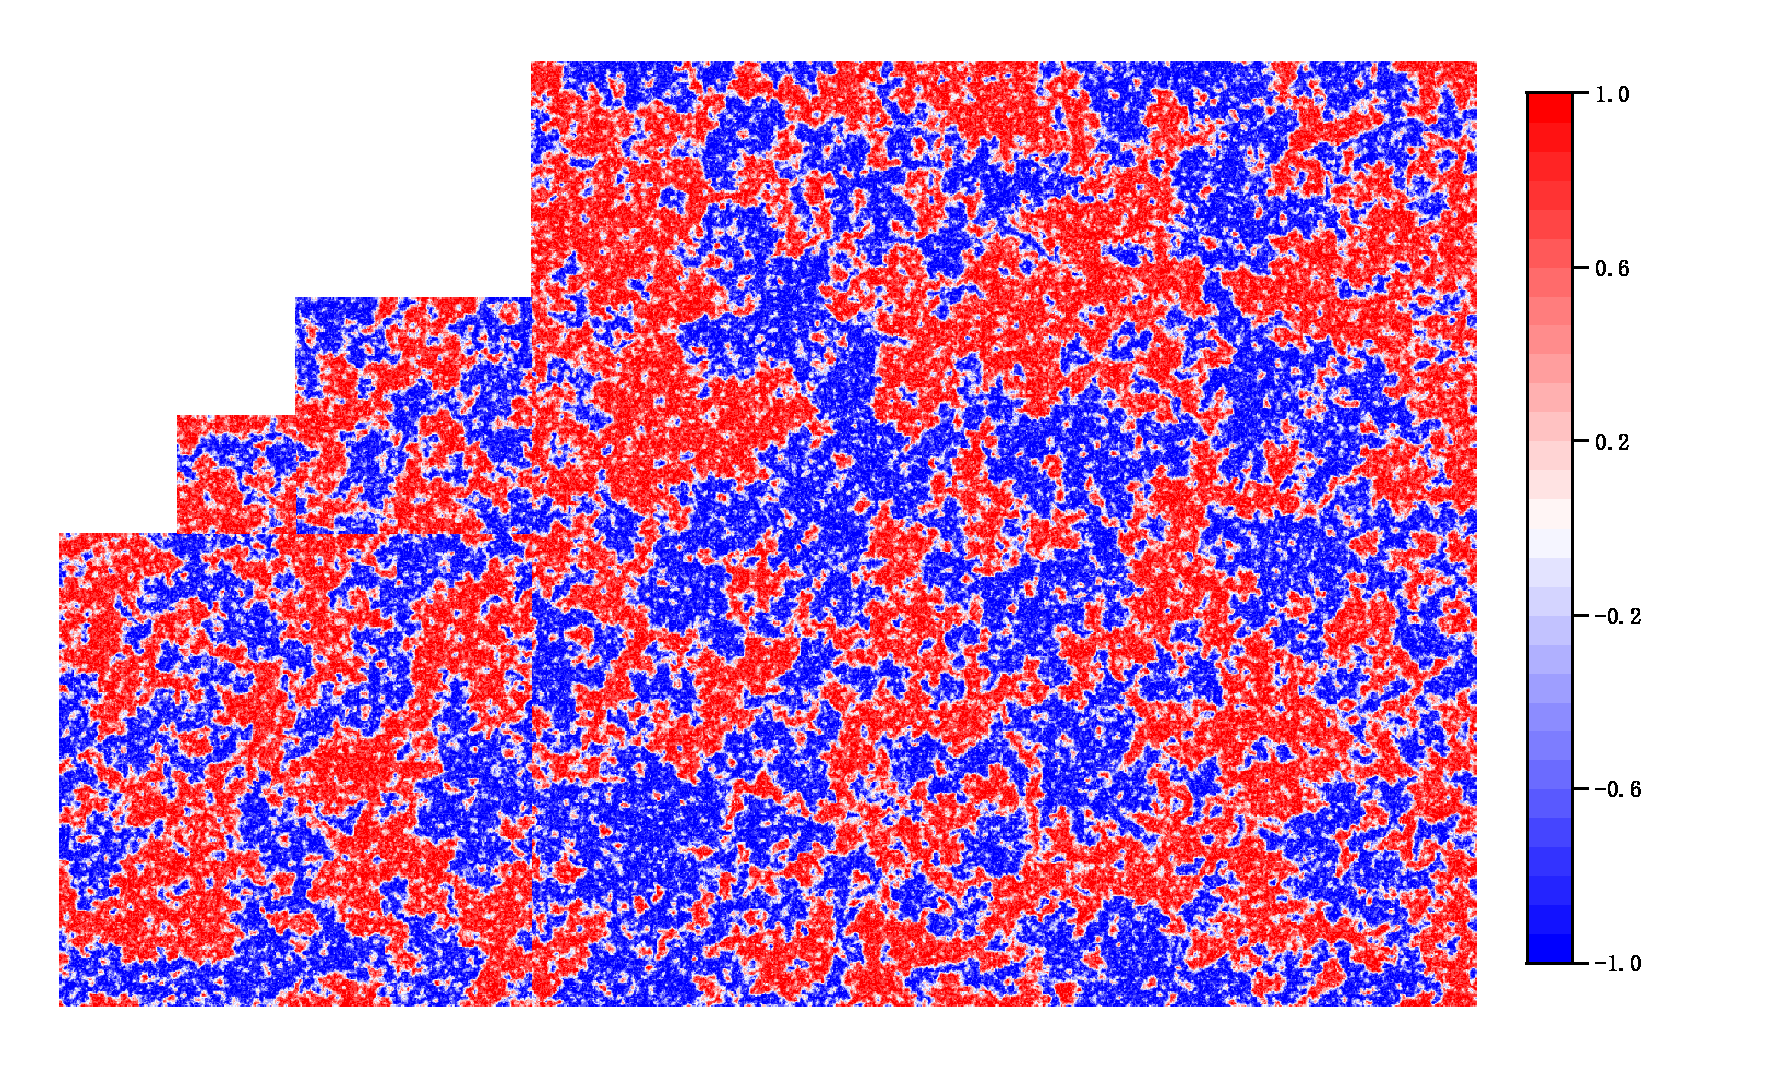
\includegraphics[width=17cm]{4_Size_Grids.pdf}
                \end{center}
                从图中可以看出磁畴尺寸基本上是随着网格大小的增大变大的, 这是由于网格的周期边界条件会影响到了大尺寸磁畴的产生, 因为周期频率很低的大磁畴是无法存在于小网格中的.
                \newpage
            \subsubsection{温度对零外场磁畴凝聚的影响}
                \indent 显然这种结构的出现于温度是息息相关的, 因为在温度较低的时候, 系统的一大块磁畴的能量足够低足够稳定, 而随着温度的升高, 这种大块的结构会因为其中的磁矩受到热激发翻转
                而被破坏, 所以大块的磁畴会逐渐分解成小块的. 以下模拟验证了这种结果:
                \begin{center}
                    \includegraphics[width=17cm]{4_T_Grids.pdf}
                \end{center}
                \newpage
            \subsubsection{平均时间对零外场磁畴凝聚的影响}
                \indent 显然这种磁畴是会随着自旋的不断翻转而逐渐产生, 消失和移动. 所以随着平均时间的增加, 自旋翻转会使得不同区域磁矩的时间平均值趋于一致.
                从模拟结果可以看出这种移动其实是十分缓慢的, 在很长一段时间内磁矩的时间平均仍然会出现局域性. 当然这种局域的尺寸会比磁畴的尺寸大很多,
                因为磁畴的移动会抹平高频的边界.
                \begin{center}
                    \includegraphics[width=17cm]{4_Num_Grids.pdf}
                \end{center}
                \newpage
        \subsection{磁滞曲线的模拟}
            \indent 由于Ising模型可以较好的模拟实际铁磁体的各种性质, 所以这里选择一种铁磁体的典型行为--磁滞曲线进行模拟.
            这里模拟的方式是:\\
            \indent 首先由随机状态达到极值磁场下的平衡态 ($T<T_c$), 即磁矩是同向的, 再逐渐步进减小磁场, 每减小一次就重新达到一次平衡, 然后记录多个个系综的平均值作为总磁矩,
            直至磁场达到反向极值, 再反过来重复以上过程. 以下是在不同温度下的模拟结果:
            \begin{center}
                \includegraphics[width=17cm]{HysteresisCurve.pdf}
            \end{center}
            可以看出与实际的磁滞曲线十分相似, 而且在高温时从铁磁介质转变为顺磁介质这种现象也十分明显.
    \section{结论}
        \indent 经过以上计算结果表明, 虽然伊辛模型是一个十分简单的解释自旋相互作用系统的模型, 但是其在不同温度下的统计规律却能反映丰富的物理内涵, 值得进行数值模拟, 以便验证系综理论的正确性.
        而这仅仅是一个简单的二维系统, 若推广到三维乃至更高维, 相信还会出现更多精细现象. 而模拟的方法梅特波斯利算法本身就是一个适用性很广的方法, 在各个领域都有应用.
\end{document}